\chapter{Reductions and Completeness}\label{chap:reduc-complete}

For polynomials, the most natural form of reductions are via \emph{projections}. 
We shall say that a polynomial $f$ \emph{reduces} to $g$ via projections if $g$ may be obtained by substituting variables of $f$ to other variables or field constants. 
Under such reductions, do we have natural complete polynomials for the classes $\VP$ and $\VNP$? 
Valiant \cite{v79} showed that the $\Det_n$ and $\Perm_n$ are (almost) complete for the classes $\VP$ and $\VNP$ respectively. 
We shall see the proof of this in this section. 

\begin{theorem}[\cite{v79}]\label{thm:vp}
If $f$ is a polynomial computed by an ABP of size $s$, then $f$ reduces to $\Det_n$ via projections for $n = \poly(s)$. 
\end{theorem}
\begin{theorem}[\cite{v79}]\label{thm:vnp}
Over any field $\F$ of characteristic not equal to $2$, the polynomial $\Perm_n$ is \emph{complete} for the class $\mathsf{VNP}$ under projections.
\end{theorem}

\section{Warm-up: Formulas to permanents}\label{sec:formula-to-dets}

Let us first show that any polynomial sized arithmetic formula can be expressed as permanent of a small matrix.
In fact, all matrices that we shall be building this way will have the following structure, and this would be
important. (Here \textcolor{red}{*}, \textcolor{blue}{*} denote upper triangle entry of the matrix of $f$, $g$ respectively.)

\begin{center}
\begin{tikzpicture}
\node at  (-1.5,1.5) {$f \quad = \quad \Perm$};
\draw (0,0) rectangle (3,3);
\node at (0.25,0.25) {1};
\node at (2.75,0.25) {0};
\node at (0.25,2.75) {0};
\node at (0.75,2.25) {1};
\node at (2.25,0.75) {1};
\draw[dotted] (2,1) -- (1,2);
\draw (0.75,2.75) -- (2.75,2.75) -- (2.75,0.75) -- cycle;
\node[text=red] at (2.1,2.1) {$\ast$};
\begin{scope}[shift={(8,0)}]
\node at  (-1.5,1.5) {$g \quad = \quad \Perm$};
\draw (0,0) rectangle (3,3);
\node at (0.25,0.25) {1};
\node at (2.75,0.25) {0};
\node at (0.25,2.75) {0};
\node at (0.75,2.25) {1};
\node at (2.25,0.75) {1};
\draw[dotted] (2,1) -- (1,2);
\draw (0.75,2.75) -- (2.75,2.75) -- (2.75,0.75) -- cycle;
\node[text=blue] at (2.1,2.1) {$\ast$};
\end{scope}
\end{tikzpicture}
\end{center}

\subsection*{Multiplication}

\begin{center}
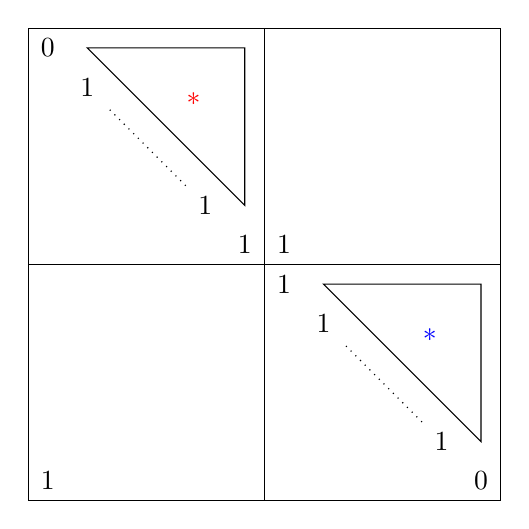
\begin{tikzpicture}
\draw (0,-3) rectangle (6,3);
\draw (0,0) rectangle (3,3);
\node at (2.75,0.25) {1};
\node at (0.25,2.75) {0};
\node at (0.75,2.25) {1};
\node at (2.25,0.75) {1};
\draw[dotted] (2,1) -- (1,2);
\draw (0.75,2.75) -- (2.75,2.75) -- (2.75,0.75) -- cycle;
\node[text=red] at (2.1,2.1) {$\ast$};
\begin{scope}[shift={(3,-3)}]
\draw (0,0) rectangle (3,3);
\node at (2.75,0.25) {0};
\node at (0.25,2.75) {1};
\node at (0.75,2.25) {1};
\node at (2.25,0.75) {1};
\draw[dotted] (2,1) -- (1,2);
\draw (0.75,2.75) -- (2.75,2.75) -- (2.75,0.75) -- cycle;
\node[text=blue] at (2.1,2.1) {$\ast$};
\end{scope}
\node at (0.25,-2.75) {1};
\node at (3.25,0.25) {1};
\end{tikzpicture}
\end{center}

\subsection*{Addition}

\begin{center}
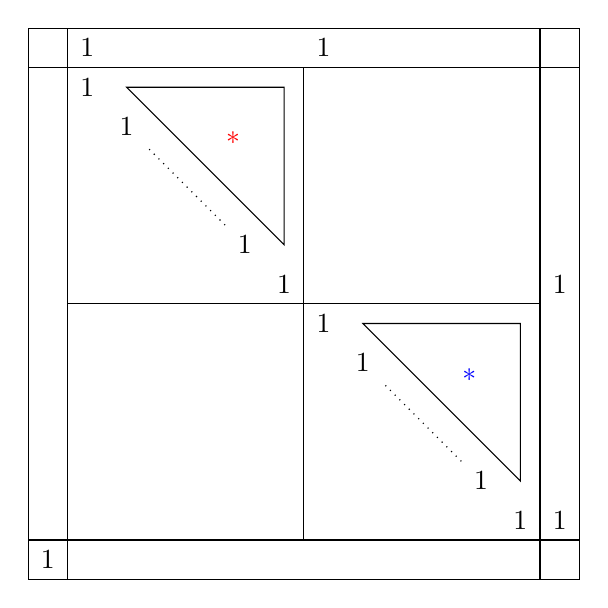
\begin{tikzpicture}

\draw (-0.5,-3.5) rectangle (0,3.5);
\draw (6,-3.5) rectangle (6.5,3.5);
\draw (6,3) rectangle (0,3.5);
\draw (0,-3.5) rectangle (6,3);

\draw (-0.5,-3) rectangle (6.5,3);
\draw (0,0) rectangle (3,3);
\node at (2.75,0.25) {1};
\node at (0.25,2.75) {1};
\node at (0.75,2.25) {1};
\node at (2.25,0.75) {1};
\draw[dotted] (2,1) -- (1,2);
\draw (0.75,2.75) -- (2.75,2.75) -- (2.75,0.75) -- cycle;
\node[text=red] at (2.1,2.1) {$\ast$};
\begin{scope}[shift={(3,-3)}]
\draw (0,0) rectangle (3,3);
\node at (2.75,0.25) {1};
\node at (0.25,2.75) {1};
\node at (0.75,2.25) {1};
\node at (2.25,0.75) {1};
\draw[dotted] (2,1) -- (1,2);
\draw (0.75,2.75) -- (2.75,2.75) -- (2.75,0.75) -- cycle;
\node[text=blue] at (2.1,2.1) {$\ast$};
\end{scope}
\node at (-0.25,-3.25) {1};
\node at (0.25,3.25) {1};
\node at (3.25,3.25) {1};
\node at (6.25,0.25) {1};
\node at (6.25,-2.75) {1};
\end{tikzpicture}
\end{center}

We leave it to as an exercise to check that this indeed works. This may seem bizarre at first but there is indeed a
method to this. To understand that method, we must realise that there is a graph theoretic way to understand $\Det_n$ and $\Perm_n$. 

\subsection*{Graph theoretic representation of $\Det_n$ and $\Perm_n$}

Let us think of an $n\times n$ symbolic matrix as an adjacency matrix of a directed graph $G$ with the edge from $i$ to $j$ having weight $x_{ij}$. 
Then every monomial of $\Det_n$ or $\Perm_n$ corresponds to a permutation $\sigma$, and the corresponding edges in the graph $G$ form a \emph{cycle cover} i.e., a partition of the vertices of $G$ into disjoint cycles. 
The weight of a cycle-cover shall be defined as the product of weights of the edges constituting the cycles, and the sign of the cycle cover shall be the sign of the permutation $\sigma$. 
This allows us to write $\Det_n$ and $\Perm_n$ as
\begin{eqnarray*}
\det(G) & = & \sum_{C\in \mathrm{CycleCovers}(G)} wt(C) \cdot \mathrm{sign}(C),\\
\mathrm{perm}(G) & = & \sum_{C\in \mathrm{CycleCovers}(G)} wt(C).\\
\end{eqnarray*}

\section{ABPs reduce to $\Det_n$}

We shall now show that for any $f$ computable by an ABP, there is a matrix  $A$ each of whose entries are either variables of constants such that $\det(A) = f$. 
Since any ABP is a projection of the polynomial $\IMM_{n,d}$, we shall show that we can construct a matrix  $A$  such that $\det(A) = \IMM_{n,d}$. \\

Consider the graph $G$ underlying the ABP that corresponds to the polynomial $\IMM_{n,d}$. 
Let $s$ and $t$ be the unique source and sink vertices respectively. 
Every path from $s\leadsto t$ corresponds to a single monomial of $\IMM_{n,d}$ of degree $d$. 
We shall now modify the graph slightly such that each such $s\leadsto t$ path would map to a unique cycle cover:

\begin{quote}
  To the graph $G$, add an edge with weight $1$ from $t$ to $s$. 

  Further, for all nodes except $s$ and $t$, add a self-loop of weight $1$. 
\end{quote}

Let $A$ be the adjacency matrix of this new graph $G'$. 
The claim is that $\det(A)$ is either $\IMM_{n,d}$ or $-\IMM_{n,d}$. 
To see this observe that all cycle covers of $G'$ must consist of a single $s\leadsto t$ path that loops back to $s$ via the edge $t\rightarrow s$ that we added, and self-loops on all excluded vertices. 
Further, since all $s\leadsto t$ paths in $G$ were of the same length, it is easy to check that all the cycle covers
have the same sign. If the sign is negative, we can change the weight of the $t\leadsto s$ edge to $-1$.
Thus $\IMM_{n,d}$ does indeed reduce to $\Det_m$ for $m = \poly(n)$. \qed {\footnotesize (\autoref{thm:vp})}\\

\begin{exercise}
Look back at the construction in \autoref{sec:formula-to-dets} to convince yourself that the permanents are indeed $f \cdot g$ and $f + g$. 

Proving the same for determinants requires handling signs. Modify the construction appropriately for determinants. 

{\bf Hint:} Convert a formula to an ABP with the property that all $s \leadsto t$ paths have the same length?
\end{exercise}

We shall soon see \cref{thm:det-abp} that $\Det_n$ can also be computed by polynomial sized ABPs and hence $\Det_n$ is complete for the class of ABPs. 

\section{Completeness of the permanent}

The $\VNP$ completeness for the permanent is trickier, and uses a very clever gadget. 
The proof described here is a modification of the proof in B\"urgisser's book \cite{bur00}. 
This is the simplest proof that I am aware of currently. \\

Let $f(x_1,\dots, x_n) = \sum_\veca g(x_1,\dots, x_n, a_1,\dots, a_m)$ be in $\VNP$ with $g(\vecx, \vecy)$ computable by a formula of size $s$ (\autoref{thm:vnp-formula}). 
Like in the previous section, we can construct a graph $G$ (with weights being either scalars or variables in $\vecx$ or $\vecy$) such that the sum of weighted cycle covers is equal to $g(\vecx, \vecy)$. 
The goal is to now compute $\sum_\veca g(\vecx, \veca)$. \\

Let us consider a simpler case, where there is a variable $y \in \vecy$ such that there is just one edge in $e_y \in G$ with weight $y$. 
Can we transform the graph $G$ locally to compute $g' = g_{(y=0)} + g_{(y=1)}$? 
Note that since $y$ occurs only once in $G$, we have that $g = y \cdot g_1 + g_0$ where $g_1$ and $g_0$ are independent of $y$. 
Thus, the polynomial $g'$ can be written as $g_1 + 2 g_0$. 
One way to compute this is to transform the graph $G$ so that any cycle-cover of $G$ that includes the edge $e_y$ has the same weight as before, but every cycle-cover that does not include the edge $e_y$ has its weight multiplied by $2$. 
This can be achieved by splitting the edge $e_y$ in the middle with a new vertex $v$ with a self-loop of weight $2$:

\begin{tikzpicture}[->,>=stealth',shorten >=1pt,auto,thick,main node/.style={circle,fill=blue!20,draw}]
\node[main node] (u) at (0,0) {};
\node[main node] (v) at (2,0) {}
edge[<-] node[above] {$y$} (u);
\node (arrow) at (4,0) {\Large $\leadsto$};
\node[main node] (u1) at (6,0) {};
\node[main node] (u2) at (7,0) {}
edge[<-] (u1);
\node[main node] (v1) at (8,0) {}
edge[<-] (u2);
\path[every node/.style={font=\tiny}] (u2) edge [loop above] node {2} (u2);
\end{tikzpicture}

Clearly, any cycle-cover that uses the edge $e_y$ has the same weight, and all other cycle-covers are forced to take the self-loop around the added vertex of weight $2$. 
This allows us to handle graphs $G$ where every variable $y \in \vecy$ occurs only once in $G$. 
The complication arises because there could be multiple edges that has the label $y$. 
We want a way by which we can say that all cycle covers that choose \emph{any} of the $y$-edges have the same weight, but cycle-covers that do not pick any $y$-edge have weight multiplied by $2$. 
The following is a gadget that has similar properties, called \emph{rosette}. 
The diagram below represents the $4$-rosette. 
\begin{center}
\begin{tikzpicture}[->,>=stealth',shorten >=1pt,auto,thick,main node/.style={circle,fill=blue!20,draw}]
\node[main node] (v1) at (0,0) {};
\node[main node] (v2) at (2,0) {};
\node[main node] (v3) at (2,2) {};
\node[main node] (v4) at (0,2) {};

\path[every node/.style={font=\tiny},ultra thick] (v1) edge (v2)
(v2) edge (v3)
(v3) edge (v4)
(v4) edge (v1);

\node[main node] (l1) at (1,-1) {};
\node[main node] (l2) at (3,1) {};
\node[main node] (l3) at (1,3) {};
\node[main node] (l4) at (-1,1) {};

\path[every node/.style={font=\tiny},thick] (l1) edge (v2)
edge [loop below] (l1)
(v2) edge (l2)
(l2) edge[loop right] (l2)
(l2) edge (v3)
(v3) edge (l3)
(l3) edge [loop above] (l3)
(l3) edge (v4)
(v4) edge (l4)
(l4) edge [loop left] (l4)
(l4) edge (v1) 
(v1) edge (l1)
(v1) edge [out=240,in=210,looseness=12] (v1)
(v2) edge [out=330,in=300,looseness=12] (v2)
(v3) edge [out=60 ,in=30 ,looseness=12] (v3)
(v4) edge [out=150,in=120,looseness=12] (v4);
\end{tikzpicture}
\end{center}
The thick edges in the above picture shall be called \emph{connector edges} (these shall play the role of the $y$-edges). 
Note that the rosette has the following two properties:
\begin{enumerate}
\item For any non-empty subset $S$ of the connector edges, there is exactly one cycle-cover of the rosette that includes exactly the set $S$ of the connector-edges. 
\item There are exactly two cycle-covers of the rosette that do not include any connector edge. 
\end{enumerate}
Thus, if we could somehow ``glue'' the connector edges with our $y$-edges, we would be done. 
This is achieved by yet another gadget that we shall call the \emph{glue gadget}. 
The following is the description of the glue gadget that glues edges $(u,v)$ and $(u',v')$ by adding three additional vertices. 

\begin{center}
\begin{tikzpicture}[->,>=stealth',shorten >=1pt,auto,thick,main node/.style={circle,fill=blue!20,draw}]
\node[main node] (u) at (0,0) {};
\node (lu) at (0,-0.5) {$u$};
\node[main node] (v) at (6,0) {};
\node (lu) at (6,-0.5) {$v$};

\node[main node] (u1) at (0,2) {};
\node (lu1) at (0,1.5) {$u'$};

\node[main node] (v1) at (6,2) {};
\node (lv1) at (6,1.5) {$v'$};

\node[main node] (p1) at (2,0) {};
\node at (2,0) {\tiny $p_1$};

\node[main node] (p2) at (4,0) {};
\node at (4,0) {\tiny $p_2$};

\node[main node] (p3) at (3,2) {};
\node at (3,2) {\tiny $p_3$};

\path[every node/.style={font=\tiny},thick] (u) edge (p1)
(p1) edge [bend left] (p2)
(p2) edge (v)
(u1) edge (p3)
(p3) edge (v1)
(p3) edge [loop above] node {$-1/2$} (p3)
(p1) edge [bend left=20] node {$1/2$} (p3)
(p2) edge [bend right=20] node [above right] {$-1/2$} (p3)
(p3) edge [bend left=20] (p1)
(p3) edge [bend right=20] (p2)
(p1) edge [loop below] node {$-1$} (p1)
(p2) edge [loop below] node {$1$} (p2)
edge [bend left=20] (p1);
\end{tikzpicture}
\end{center}
The adjacency matrix between the nodes $p_1$, $p_2$ and $p_3$ is 
\[
A = \insquare{\begin{array}{rrr}
-1 & 1 & 1/2\\
1 & 1 & -1/2\\
1 & 1 & -1/2
\end{array}}.
\]

\noindent
\begin{claim}
Let $(u,v)$ and $(u',v')$ be two edges of a graph $G$, and let $G'$ be the graph with the glue gadget between them as described above. 
Then $\mathrm{perm}(G')$ equals the sum of all weighted cycle covers of $G$ that either include both $(u,v)$ and $(u',v')$ in it or neither. 
\end{claim}
\begin{proof}
If both edges $(u,v)$ and $(u',v')$ are taken in the cycle cover, this is realized in $G'$ as ${(\ldots u,p_1, p_2, v \ldots) (\ldots u', p_3, v' \ldots)}$, which has the same weight.  

If neither of the edges $(u,v)$ and $(u',v')$ are taken in the cycle cover, then the total contribution of all cycle covers of $p_1$, $p_2$ and $p_3$ is $\mathrm{perm}(A) = 1$. 

If the edge $(u,v)$ is taken but $(u',v')$ is not, then the edge $(u,v)$ can be realized in $G'$ as either $\inbrace{(\ldots u,p_1,p_2,v \ldots) (p_3)}$ or $\inbrace{(\ldots u,p_1,p_3,p_2,v \ldots )}$. 
The total contribution is therefore zero. 

Similarly, if the edge $(u',v')$ is taken but not $(u,v)$, then this can be realized in $G'$ as $\inbrace{(\ldots u',p_3,v' \ldots),(p_1,p_2)}$ and $\inbrace{(\ldots u',p_3, v' \ldots) (p_1) (p_2)}$. 
Again, the net contribution is zero.  
\end{proof}

Now with these two gadgets, we are done. 
For every variable $y_i \in \vecy$, let $e_{i,1}, \dots, e_{i,r_i}$ be the edges labelled with $y$. 
Let $R_i$ be a $r_i$-rosette disjoint from the graph $G$ The graph $G'$ is built as follows:
\begin{quote}
  Take a disjoint union of $G$ with one $r_i$-rosette for each $i = 1,\dots, m$. 

  Glue each edge labelled with $y_i$ with the $r_i$ connector edges in the $r_i$-rosette. 
\end{quote}

It should be easy to see that $\mathrm{perm}(G) = \sum_{\veca} g(\vecx, \veca)$. 
This completes the proof of the $\VNP$-completeness of $\Perm_n$. \qed {\footnotesize (\autoref{thm:vnp})} \\

Note that we needed to divide by $2$ in the glue gadget. 
This is why we require the characteristic of the field to be different from two for the above proof to work. 

\begin{exercise}
  For any matrix $A$, we shall use the notation that $A[1|2]$ refers to the submatrix obtained by removing row $1$ and column $2$.

  Show that, for a three-vertex \emph{glue gadget}, it suffices to find a $3\times 3$ matrix $A$ that satisfies the following three properties:
  \begin{itemize}
    \item $\mathrm{perm}(A) = \mathrm{perm}(A[2,3|1,3]) = 1$. 
    \item $\mathrm{perm}(A[3|3]) = \mathrm{perm}(A[2|1]) = \mathrm{perm}(A[1|3]) = \mathrm{perm}(A[2|3]) = 0$.
  \end{itemize}
  
  Come up with an alternate construction of a matrix $A$ as a \emph{glue gadget}. 
Also prove that any such construction must involve entries of $A$ with its denominator divisible by $2$, and show that replacing $\mathrm{perm}$ by $\det$ above would yield no solution. 
\end{exercise}


%%% Local Variables: 
%%% mode: latex
%%% TeX-master: "fancymain"
%%% End: 
